% PSI Beamer presentation: LESTO Task 3.4 progress for the project partners.
% Every number on a slide comes from a repository file: manuscript/generated
% (numbers.tex, results.json, the generated tables), the manuscript
% sections, run/023 and run/024 records, deliverables/D38/main.tex.
% Figures and their inputs: figure_sources.json (make_figures.py).
% The PSI theme files and assets are copied from presentations/case-ladder.
\PassOptionsToPackage{table}{xcolor}
\documentclass[aspectratio=169,10pt]{beamer}
\usetheme{PSI}
\usepackage{amsmath,amssymb}
\usepackage{booktabs,array}
\usetikzlibrary{positioning}
\ifXeTeX
  \setsansfont{Liberation Sans}
  \setmonofont{Liberation Mono}
\fi
\ifLuaTeX
  \setsansfont{Liberation Sans}
  \setmonofont{Liberation Mono}
\fi
\graphicspath{{figures/}{psi-assets/}{./}}
\setbeameroption{hide notes}
\setbeamerfont{title}{size=\fontsize{20}{25}\selectfont,series=\bfseries}
\setbeamerfont{subtitle}{size=\fontsize{14}{18}\selectfont,series=\mdseries}
\setbeamerfont{section page}{size=\fontsize{26}{31}\selectfont,series=\bfseries}
\renewcommand{\PSIfootername}{PSI \enspace | \enspace LESTO Task 3.4 \enspace | \enspace Partner update}
\renewcommand{\PSIfootdate}{15.10.2026}

\title{CFD--GEMS3K modelling of\\iodine transport and deposition}
\subtitle{LESTO Task 3.4 progress}
\author{Jan Kren, with Bojan Ničeno}
\institute{LESTO Task 3.4 \enspace | \enspace Villigen PSI}
\date{15 October 2026}
\psititlestyle{blue}

\setbeamercolor{keybox}{fg=PSIblack,bg=PSIblue!8}
\newcommand{\PbI}{PbI\textsubscript{2}}
\newcommand{\BiI}{BiI\textsubscript{3}}
\newcommand{\subhead}[1]{{\normalsize\bfseries\color{PSIblack}#1\par}\vspace{0.15em}}
% one-line take-home message under a slide title
\newcommand{\key}[1]{\begin{beamercolorbox}[sep=0.35em,wd=\linewidth]{keybox}\small\raggedright\textbf{#1}\end{beamercolorbox}\vspace{0.3em}}
\newcommand{\figsrc}[1]{\par\vspace{0.1em}{\raggedright\footnotesize\color{PSIgray}#1\par}}
\setlength{\leftmargini}{1.0em}
\AtBeginEnvironment{itemize}{\small\setlength{\itemsep}{2pt}}
\tikzset{
  lad/.style={draw=#1,fill=#1!10,rounded corners=1.5pt,minimum width=0.95cm,minimum height=0.6cm,inner sep=1pt,font=\small\bfseries},
  bk/.style={->,>=stealth,line width=0.6pt,draw=PSIgray},
  blk/.style={draw=#1,fill=#1!8,rounded corners=2pt,align=center,font=\footnotesize,inner sep=3pt,text width=4.0cm,minimum height=0.7cm}}
\colorlet{cCarrier}{PSIblue}
\colorlet{cSpecies}{PSIpurple}
\colorlet{cExchange}{PSIred}
\colorlet{cBench}{PSIgreen!55!black}

\begin{document}

% 1 title -----------------------------------------------------------------
{\setbeamertemplate{footline}{}\setbeamertemplate{headline}{}
\begin{frame}[plain]
  \titlepage
  \note{(0.5 min) Progress of the PSI part of Task 3.4: a CFD model of iodine transport and deposition, coupled to the GEMS3K chemical-equilibrium code, tested against thermal-gradient column experiments. The solver groundwork, the carrier-flow and species-transport cases, is Bojan Ničeno's; he is also co-author of the manuscript.}
\end{frame}}

% 2 why -------------------------------------------------------------------
\begin{frame}[t]{From column experiments to the reactor hall}
  \key{Task 3.4: fission products from the source into the reactor hall}
  \begin{columns}[T,onlytextwidth]
    \begin{column}{0.50\textwidth}
      \subhead{Why thermal-gradient columns}
      \begin{itemize}
        \item volatile iodine compounds released from LBE travel with a gas and deposit where they become supersaturated
        \item columns do this under control: known gas flow, measured wall temperature, measured deposit along the tube
        \item a model that reproduces them has its transport, wall exchange and chemistry tested together
      \end{itemize}
    \end{column}
    \begin{column}{0.46\textwidth}
      \subhead{Where this tool fits in the task}
      \begin{itemize}
        \item PSI: CFD (OpenFOAM) coupled with GEMS chemical equilibrium; experiments; later machine learning
        \item SCK CEN: a comparative approach, HSC Chemistry with Fluent
        \item CIRTEN: reduced-order models
        \item VKI is also a partner of the task
      \end{itemize}
      {\small\color{PSIgray}This talk: the PSI CFD--GEMS3K model and what it can offer to the other approaches.\par}
    \end{column}
  \end{columns}
  \note{(2 min) The task goal is the source term: how much iodine and other fission products leave the coolant and where they go in the reactor hall. Before a model is trusted in a reactor geometry, it has to reproduce a controlled experiment. Thermal-gradient columns, also called thermochromatography or thermosublimatography, are exactly that: a known helium flow carries the evaporated compounds along a falling wall temperature and the deposit is scanned along the tube. Within the task, PSI couples CFD with GEMS chemistry; SCK CEN follows a comparative approach with HSC Chemistry and Fluent; CIRTEN works on reduced-order models. The second half of the talk says what we can offer to these approaches.}
\end{frame}

% 3 experiments -----------------------------------------------------------
\begin{frame}[t]{Two sets of published column experiments}
  \key{Eight experiments with measured wall temperature and deposit scans}
  \begin{columns}[T,onlytextwidth]
    \begin{column}{0.42\textwidth}
      \subhead{Liu et al.\ (2025), PSI}
      \begin{itemize}
        \item 1.25 m columns: steel (4.8 mm) and silica (5.0 mm)
        \item pure \PbI{}; iodine in LBE at 900\,$^\circ$C
        \item helium 45 or 100 mL/min, 3 h; 1 cm scans
      \end{itemize}
      \subhead{Lobresco et al.\ (2026)}
      \begin{itemize}
        \item five pure \PbI{} experiments: 5--540 mL/min, 6--300 s
      \end{itemize}
    \end{column}
    \begin{column}{0.55\textwidth}
      \centering
      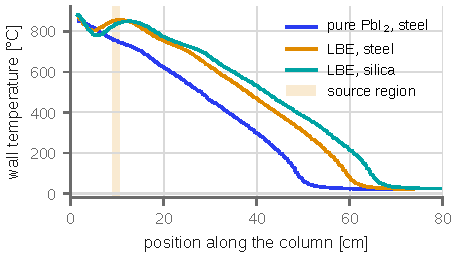
\includegraphics[width=\linewidth]{temperature_profiles}
      \figsrc{Digitised from Liu et al.\ (2025)}
    \end{column}
  \end{columns}
  \note{(2 min) Liu et al. measured three configurations we can rebuild: pure PbI2 in steel and iodine-containing LBE in steel and silica; a fourth, BiI3 in silica, has no published temperature profile and is not run. The source sits in a hot furnace and helium carries the vapour down a falling temperature. Lobresco et al. published five single-compound PbI2 experiments with flows from 5 to 540 mL per minute; their digitised data are CC BY 4.0. All our inputs come from the published figures; the source release history, the flow reference conditions and the coordinate origin are not published and are assumptions.}
\end{frame}

% 4 model, transport ------------------------------------------------------
\begin{frame}[t]{Model, part 1: transport and wall exchange}
  \key{Trace gases in laminar helium; a conservative law for the wall}
  \begin{columns}[T,onlytextwidth]
    \begin{column}{0.48\textwidth}
      \begin{itemize}
        \item OpenFOAM finite volumes, axisymmetric 5$^\circ$ wedge of the column
        \item laminar helium carrier ($\mathrm{Re}\approx0.7$--3), computed once and frozen
        \item vapours are dilute traces carried and diffusing in it
        \item wall exchange: Hertz--Knudsen--Schrage evaporation/condensation law in series with diffusion to the wall
        \item condensed material is stored in wall inventories that can evaporate again
      \end{itemize}
    \end{column}
    \begin{column}{0.48\textwidth}
      \centering
      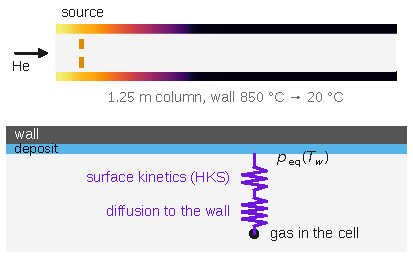
\includegraphics[width=\linewidth]{model_sketch}
      \figsrc{Resistances in series; wall $T$ of the \PbI{} steel column}
    \end{column}
  \end{columns}
  \note{(2 min) The carrier is laminar, the Reynolds number is about 0.7 to 3, so the helium flow is computed once with the measured wall temperature and then frozen. The vapours are traces in it. At the wall, condensation and evaporation follow the Hertz-Knudsen-Schrage law, driven by the difference between the gas partial pressure and the equilibrium vapour pressure at the wall temperature. The important detail: the solver does not apply that law at the cell centre but puts it in series with the diffusion resistance between the cell centre and the wall. Deposited material stays on the wall as an inventory and can evaporate again when conditions change.}
\end{frame}

% 5 model, chemistry ------------------------------------------------------
\begin{frame}[t]{Model, part 2: chemistry with GEMS3K}
  \key{Nine Pb--Bi--I gases re-equilibrate in every cell; no atom is lost}
  \begin{columns}[T,onlytextwidth]
    \begin{column}{0.48\textwidth}
      \begin{itemize}
        \item gases: Pb, PbI, \PbI{}, Bi, Bi\textsubscript{2}, BiI, \BiI{}, I, I\textsubscript{2}
        \item condensed: \PbI{}, \BiI{}, Pb, Bi on the wall
        \item each step: transport, then local gas equilibrium at fixed element amounts of Pb, Bi and I
        \item GEMS3K (PSI's Gibbs-energy minimisation code) linked into the solver through a small C bridge
        \item an element ledger checks every atom
      \end{itemize}
    \end{column}
    \begin{column}{0.48\textwidth}
      \centering
      \begin{tikzpicture}[node distance=0.4cm]
        \node[blk=PSIblue] (of) {\textbf{OpenFOAM}\\transport, wall exchange};
        \node[blk=PSIpurple,below=of of] (br) {\textbf{C bridge}\\element amounts, $T$, $p$};
        \node[blk=PSIred,below=of br] (gm) {\textbf{GEMS3K}\\equilibrium, vapour pressures};
        \draw[bk,<->] (of) -- (br);
        \draw[bk,<->] (br) -- (gm);
      \end{tikzpicture}
      \figsrc{Function calls in memory, no file exchange per step.}
    \end{column}
  \end{columns}
  \note{(2 min) Nine gases cover lead, bismuth and iodine. After each transport step the gas in every cell is brought to equilibrium at its current element amounts, so speciation follows temperature along the column, while the number of lead, bismuth and iodine atoms stays exactly what transport delivered. GEMS3K is PSI's Gibbs-energy minimisation kernel; it is linked statically into the OpenFOAM executable through a plain C bridge. It can supply the equilibrium vapour pressures of the wall law and the gas standard states for the speciation. An element ledger books every transfer between gas, wall and outlet.}
\end{frame}

% 6 ladder ----------------------------------------------------------------
\begin{frame}[t]{Built step by step: 24 test cases}
  \key{Every capability has a case that isolates it and a number that checks it}
  \centering
  \begin{tikzpicture}[x=1.2cm,y=1.05cm]
    \foreach \n [count=\i from 0] in {001,002,003,004,005,006,007}
      \node[lad=cCarrier] (n\n) at (\i,0) {\n};
    \foreach \n [count=\i from 7] in {008,009,010,011}
      \node[lad=cSpecies] (n\n) at (\i,0) {\n};
    \foreach \a/\b in {001/002,002/003,003/004,004/005,005/006,006/007,007/008,008/009,009/010,010/011}
      \draw[bk] (n\a) -- (n\b);
    \node[lad=cExchange] (n012) at (10,-1.25) {012};
    \node[lad=cExchange] (n013) at (9,-1.25) {013};
    \node[lad=cExchange] (n014) at (8,-1.25) {014};
    \node[lad=cExchange] (n016) at (7,-1.25) {016};
    \node[lad=cExchange] (n017) at (6,-1.25) {017};
    \node[lad=cExchange] (n015) at (9,-2.5) {015};
    \node[lad=cExchange] (n018) at (8,-2.5) {018};
    \node[lad=cExchange] (n019) at (7,-2.5) {019};
    \node[lad=cExchange] (n020) at (7,-3.6) {020};
    \node[lad=cExchange] (n021) at (6,-2.5) {021};
    \node[lad=cBench] (n022) at (10,-2.5) {022};
    \node[lad=cBench] (n023) at (5,-1.25) {023};
    \node[lad=cBench] (n024) at (5,-2.5) {024};
    \draw[bk] (n011) -- (n012);
    \foreach \a/\b in {012/013,013/014,014/016,016/017,017/023,013/015,014/018,018/019,019/020,019/021,021/024,012/022}
      \draw[bk] (n\a) -- (n\b);
    \draw[bk,dashed] (n017) -- (n024);
    \node[anchor=north west,align=left,font=\small,text width=5.4cm] at (-0.45,-0.75) {%
      \textcolor{cCarrier}{\rule{7pt}{7pt}} helium flow 001--007\\
      \textcolor{cSpecies}{\rule{7pt}{7pt}} species transport 008--011\\
      \hspace*{1.0em}{\color{PSIgray}groundwork by Bojan Ničeno}\\[0.25em]
      \textcolor{cExchange}{\rule{7pt}{7pt}} wall exchange, chemistry 012--021\\
      \textcolor{cBench}{\rule{7pt}{7pt}} experiments 022--024\\[0.25em]
      {\color{PSIgray}each case: a readme, \texttt{./Allrun}, a check}};
  \end{tikzpicture}
  \note{(1 min) The code was built as a ladder of test cases in the repository. Each case is based on the one before and changes one thing: first the helium flow and species transport, Bojan Ničeno's groundwork, then the wall laws, the second iodide, the gas chemistry, the metal vapour, and finally the two experimental studies, 023 for Lobresco and 024 for Liu. Every case has a short readme and one command that reruns it and reports whether its check passes. This is also how we would hand cases to partners.}
\end{frame}

% 7 verified --------------------------------------------------------------
\begin{frame}[t]{Verified: wall law and conservation}
  \key{The wall law is second-order accurate; element balances close at round-off}
  \begin{columns}[T,onlytextwidth]
    \begin{column}{0.42\textwidth}
      \subhead{Wall law against an exact solution}
      \begin{itemize}
        \item pipe flow with wall uptake (Graetz--Robin), exact decay rate
        \item half-cell wall law: observed order 1.99--2.00
        \item law at the cell centre: order 1.004--1.008, 100$\times$ larger errors
      \end{itemize}
      \subhead{Conservation}
      \begin{itemize}
        \item worst element residue: $1.41\times10^{-12}$ of the supplied material (19 production runs)
      \end{itemize}
    \end{column}
    \begin{column}{0.55\textwidth}
      \centering
      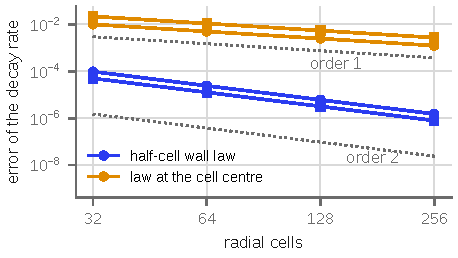
\includegraphics[width=\linewidth]{graetz}
      \figsrc{45 runs; exact reference}
    \end{column}
  \end{columns}
  \note{(2 min) Two kinds of checks. First, the wall law against a problem with a known answer: developed laminar pipe flow with uptake at the wall, the extended Graetz problem with a Robin wall condition. The decay rate of the gas along the pipe is known to twelve digits. Our half-cell law converges at second order; applying the same kinetic law at the cell centre, as a simple first-cell sink would, is only first order and about a hundred times less accurate on the same mesh. Second, conservation: in all production runs, the worst element residue is about one part in a trillion of the supplied material. Note: this verifies the numerics, not the physics.}
\end{frame}

% 8 regime ----------------------------------------------------------------
\begin{frame}[t]{Deposition is limited by diffusion}
  \key{Both limits appear; the columns sit on the diffusion side}
  \begin{columns}[T,onlytextwidth]
    \begin{column}{0.42\textwidth}
      \begin{itemize}
        \item Da: surface conductance over diffusion to the wall
        \item small Da: kinetics decide; large Da: diffusion limit $\pi^2/4$
        \item onset stays at 561\,K: saturation sets it
        \item columns: Da $\approx$ 1.4--2.9$\times10^3$ ($\alpha$ = 1), 76--150 (0.1), 7--15 (0.01)
      \end{itemize}
      \vspace{0.2em}
      {\small\textbf{So:} the sticking coefficient hardly matters; diffusivity, wall temperature and vapour pressure do.\par}
    \end{column}
    \begin{column}{0.55\textwidth}
      \centering
      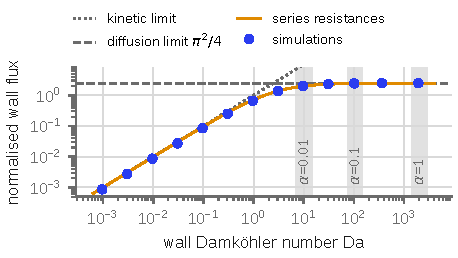
\includegraphics[width=\linewidth]{damkohler}
      \figsrc{Test channel, 13 runs; grey: the column cases}
    \end{column}
  \end{columns}
  \note{(1.5 min) Which of the two resistances controls deposition? We varied only the accommodation coefficient, which sets the surface kinetics, over six decades in a test channel. At small Damköhler number the wall flux equals Da: kinetics decide. At large Da it levels off at the diffusion limit of the channel, pi squared over four, and in between it follows the two resistances in series. The column experiments, with accommodation 1, 0.1 or 0.01, lie on the plateau or at its edge: transport to the wall is the bottleneck. For modelling partners this is useful: an uncertain sticking coefficient matters little here, while the diffusivity, the wall temperature and the vapour pressure matter a lot. The onset of deposition does not move at all, because saturation fixes it.}
\end{frame}

% 8b inside the column -----------------------------------------------------
\begin{frame}[t]{Inside the column: the wall stays saturated}
  \key{The gas next to the wall is at equilibrium; the core carries the excess}
  \begin{columns}[T,onlytextwidth]
    \begin{column}{0.42\textwidth}
      \begin{itemize}
        \item saturation: vapour over its equilibrium value at the wall temperature
        \item deposit starts where the mean reaches saturation (35.7 cm, 372\,$^\circ$C)
        \item in the deposit zone: next to the wall $\le1.009$, mean up to 1.64, axis up to 2.03
      \end{itemize}
      \vspace{0.2em}
      {\small\textbf{So:} uptake waits for diffusion; the supersaturated core is where aerosols could form, which the model leaves out.\par}
    \end{column}
    \begin{column}{0.55\textwidth}
      \centering
      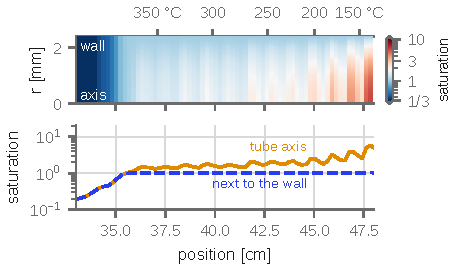
\includegraphics[width=\linewidth]{field}
      \figsrc{Pure \PbI{}, steel, 60 s; production case, 41,472 cells}
    \end{column}
  \end{columns}
  \note{(1.5 min) The same result, seen inside the pure PbI2 column. The colour is the saturation of the vapour: its amount divided by the equilibrium amount at the local wall temperature. Upstream the gas is unsaturated and nothing deposits. The deposit starts exactly where the mean reaches saturation. From there on, the gas next to the wall stays at equilibrium, within one percent, while the centre of the tube becomes more and more supersaturated, about two times on the axis. A finer upwind run gives the same picture. The wall takes everything diffusion brings, so diffusion sets the rate. The supersaturated core is also where real aerosols could nucleate; the model does not represent that, and it is on the list of open points. The ripples come from the digitised wall temperature.}
\end{frame}

% 9 sensitivities ---------------------------------------------------------
\begin{frame}[t]{What matters for the deposit}
  \key{Diffusivity, temperatures and thermodynamic data matter; kinetics does not}
  \begin{columns}[T,onlytextwidth]
    \begin{column}{0.46\textwidth}
      {\small Change of the iodine wall profile ($L_1$, \%):\par}
      \vspace{0.3em}
      \footnotesize
      \begin{tabular}{@{}>{\raggedright\arraybackslash}p{0.66\linewidth}r@{}}
        \toprule
        diffusivity halved or doubled & up to 16.65 \\
        flow reference 273 vs 298\,K & up to 10.93 \\
        silica temperature curve shifted 4.1--4.65\,cm & 187--194 \\
        BiI(g) data: \BiI{} share of iodine & 94.6 $\rightarrow$ 2.0\,\% \\
        \midrule
        accommodation 0.1 or 0.01 & at most 5.14 \\
        source moved $\pm$1.5\,cm & at most 0.19 \\
        \bottomrule
      \end{tabular}
    \end{column}
    \begin{column}{0.51\textwidth}
      \centering
      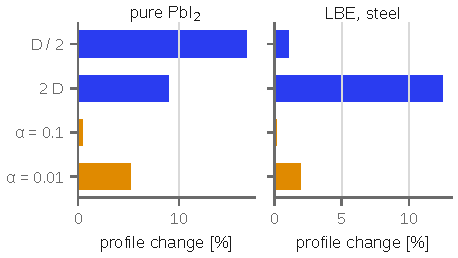
\includegraphics[width=\linewidth]{sensitivity}
      \figsrc{Two cases repeated with the production scheme}
    \end{column}
  \end{columns}
  \note{(2 min) A structured set of input variations, each compared with its own baseline. Diffusivity and the flow reference conditions shift the profiles by ten to seventeen percent. Shifting the silica temperature curve by about four centimetres moves the deposits almost completely, so the temperature input and its coordinate dominate. The thermodynamic data decide the chemistry, on the next slides. By contrast, accommodation changes the profiles by at most about five percent and moving the source region by 1.5 centimetres changes almost nothing. The figure shows the diffusivity and accommodation variations repeated with the production numerical scheme; total deposits change by less than 0.02 percent in all of them, only the shape moves.}
\end{frame}

% 10 Lobresco -------------------------------------------------------------
\begin{frame}[t]{Lobresco et al.: onset within 18 K}
  \key{Five \PbI{} experiments, untuned: onset RMS 18 K; both published models 35 K}
  \begin{columns}[T,onlytextwidth]
    \begin{column}{0.42\textwidth}
      \begin{itemize}
        \item no parameter fitted to these data
        \item onset: 1\,\% of the deposit peak, as in the paper
        \item computed peaks lie 1--4\,cm upstream
        \item carrier, vapour pressure and source differ from the published models
      \end{itemize}
      \vspace{0.2em}
      {\small\textbf{Promising, conditional:} not yet attributable to the wall law alone.\par}
    \end{column}
    \begin{column}{0.55\textwidth}
      \centering
      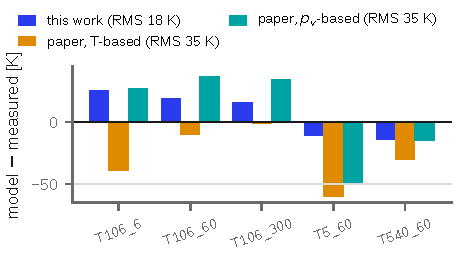
\includegraphics[width=\linewidth]{lobresco_onset}
      \figsrc{Data and models: Lobresco et al.\ (2026), CC BY 4.0}
    \end{column}
  \end{columns}
  \note{(2 min) On the five single-compound experiments of Lobresco and co-workers, run without any adjustment, our onset temperatures deviate by 18 kelvin RMS from the measurements; the two models of that paper by 35 kelvin each. Two caveats keep this a promising but conditional result. The peaks of our profiles sit one to four centimetres upstream of the measured ones. And our carrier, vapour-pressure data and source treatment differ from those of the published models, so we cannot yet say the improvement comes from the wall law. For the 5 mL per minute case the onset is taken on the main deposit; from the inlet the rule picks a small upstream deposit.}
\end{frame}

% 11 Liu steel ------------------------------------------------------------
\begin{frame}[t]{Liu et al.: the steel columns}
  \key{\PbI{} peak 366.5\,$^\circ$C (measured 368\,$\pm$\,18\,$^\circ$C); both LBE bands}
  \centering
  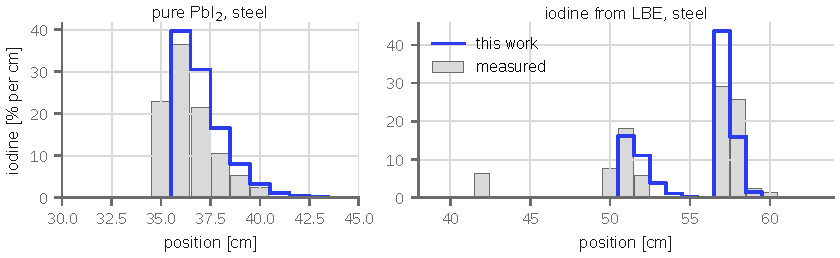
\includegraphics[width=0.98\linewidth]{liu_profiles}
  \figsrc{Measured scan adapted from Liu et al.\ (2025). Right: a \PbI{} band near 51 cm, a \BiI{} band near 57 cm.}
  \note{(2 min) In the steel columns the model reproduces the deposit positions. For pure PbI2 the computed peak is at 36 centimetres and 366.5 degrees, against 368 plus or minus 18 measured. For iodine evaporated from LBE the measurement shows two bands; the model gives both, the upstream one as PbI2 and the downstream one as BiI3. The small deposit near 42 centimetres in the measurement is not reproduced. The runs cover 60 seconds at the mean release rate of the three-hour experiment; the time history of the release is not known.}
\end{frame}

% 12 Liu silica -----------------------------------------------------------
\begin{frame}[t]{Liu et al.: the silica column}
  \key{The printed peak temperatures do not match the printed temperature curve}
  \begin{columns}[T,onlytextwidth]
    \begin{column}{0.42\textwidth}
      \begin{itemize}
        \item published curve: computed bands 4--5\,cm downstream
        \item printed peak labels (306, 127\,$^\circ$C) sit 4.1--4.65\,cm off the curve
        \item curve shifted by that: overlap 6\,\% $\rightarrow$ 73--78\,\%
        \item a hypothesis, not a result: the thermocouple data would settle it
      \end{itemize}
    \end{column}
    \begin{column}{0.55\textwidth}
      \centering
      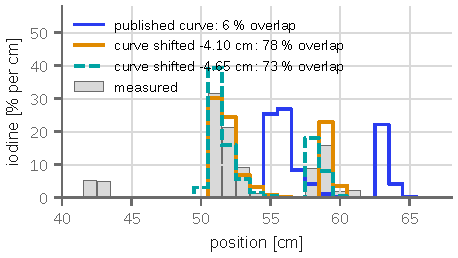
\includegraphics[width=\linewidth]{silica}
      \figsrc{Published data adapted from Liu et al.\ (2025)}
    \end{column}
  \end{columns}
  \note{(1.5 min) In the silica column the computed bands lie four to five centimetres downstream of the measured ones. The paper prints the temperatures of the two peaks; on the digitised temperature curve these temperatures occur 4.1 to 4.65 centimetres away from the printed positions. Shifting the curve by that amount moves the computed bands onto the measured ones; the overlap rises from 6 to about 75 percent. We present this as an inconsistency of the published input, not as a fit; the original thermocouple table and scan coordinates would resolve it.}
\end{frame}

% 13 thermodynamics -------------------------------------------------------
\begin{frame}[t]{Thermodynamic data decide the iodide}
  \key{One BiI(g) value moves the \BiI{} share of iodine from 94.6 to 2.0\,\%}
  \begin{columns}[T,onlytextwidth]
    \begin{column}{0.42\textwidth}
      \begin{itemize}
        \item baseline data vs BiI(g) shifted by $+29$\,kJ/mol
        \item steel, 1\,\% metal saturation: 94.58 vs 2.01\,\%
        \item the same at every tested resolution
        \item not an uncertainty band: qualified Bi--I data are needed
      \end{itemize}
    \end{column}
    \begin{column}{0.55\textwidth}
      \centering
      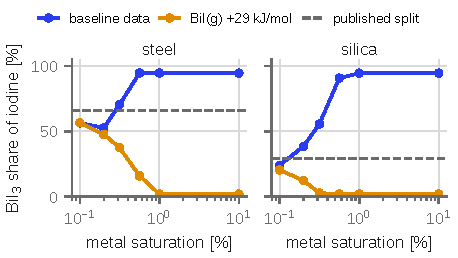
\includegraphics[width=\linewidth]{thermodynamics}
      \figsrc{LBE with added metal vapour; published split: Liu et al.\ (2025)}
    \end{column}
  \end{columns}
  \note{(1.5 min) The partition between PbI2 and BiI3 is controlled by the thermodynamic input, not by the transport. The plus 29 kilojoules per mole branch is a surrogate perturbation of the uncertain BiI gas data, not a second qualified dataset; it turns a BiI3-dominated deposit into a PbI2-dominated one. The dashed lines are the published split. This is a sensitivity, not an uncertainty interval. For the task it means that qualified thermodynamic records for the Bi-I system are as important as the transport model, and a natural point of collaboration.}
\end{frame}

% 14 D38 ------------------------------------------------------------------
\begin{frame}[t]{D38: the coupled tool and what it offers}
  \key{GEMS3K in every cell at production scale; cases to share}
  \begin{columns}[T,onlytextwidth]
    \begin{column}{0.48\textwidth}
      \subhead{Status}
      \begin{itemize}
        \item D38 (M24): the coupled GEMS and CFD codes, description of the coupling and modelling; draft ready
        \item production case with GEMS3K data in every cell: profiles change by at most $2.1\times10^{-4}$
        \item $5.1\times10^{8}$ GEMS3K calls, none failed
      \end{itemize}
    \end{column}
    \begin{column}{0.48\textwidth}
      \subhead{What we can offer}
      \begin{itemize}
        \item reference cases with measured inputs for comparative CFD, e.g.\ with HSC Chemistry and Fluent
        \item reference and training data for reduced-order models
        \item a verified wall-exchange law and a conservative coupling, documented case by case
      \end{itemize}
    \end{column}
  \end{columns}
  \note{(2 min) Deliverable D38, due at month 24, describes the coupled GEMS and CFD code; the draft is written. In a production case GEMS3K was called in every cell and step, about half a billion calls without a failure, and the deposit profiles agree with the reference to two parts in ten thousand. What can we offer? The cases with their measured inputs could serve as common reference cases for the comparative CFD approach, and the runs could provide reference or training data for reduced-order models. These are offers to discuss, not commitments.}
\end{frame}

% 15 limitations ----------------------------------------------------------
\begin{frame}[t]{What the model does not yet cover}
  \key{A conservative, verified method; not yet independent predictive validation}
  \begin{columns}[T,onlytextwidth]
    \begin{column}{0.48\textwidth}
      \subhead{Inputs}
      \begin{itemize}
        \item release history, flow reference conditions and coordinate origins are assumed
        \item near the source the vapour mole fraction reaches 0.33--0.36: not dilute there
        \item boat and end of the experiment (cooling, withdrawal) not simulated
      \end{itemize}
    \end{column}
    \begin{column}{0.48\textwidth}
      \subhead{Physics and numerics}
      \begin{itemize}
        \item frozen carrier: no buoyancy; Richardson number up to about 1.2 in the steepest section
        \item no aerosols, no thermophoresis
        \item mesh: one case refined with the production scheme (1.98\,\%); with upwind four cases change by 2.13--7.30\,\%
      \end{itemize}
    \end{column}
  \end{columns}
  \note{(1.5 min) Honest limits. The experiments do not publish the release history, the flow reference conditions or the coordinate origin, so these are assumptions. Next to the source the vapour is not dilute, which the frozen-carrier model assumes. The carrier is frozen, so buoyancy is not represented; with Richardson numbers up to about one this may matter locally if the column was horizontal, which we do not know. Aerosol formation is outside the model. Numerically, only one case was refined to the finest mesh with the production scheme, and no formal grid-convergence index is claimed.}
\end{frame}

% 16 needs ----------------------------------------------------------------
\begin{frame}[t]{Where partners could help}
  \key{Data and comparisons on common cases would turn this into a validation}
  \begin{columns}[T,onlytextwidth]
    \begin{column}{0.48\textwidth}
      \subhead{Data}
      \begin{itemize}
        \item measured wall-temperature tables and scan coordinates
        \item release histories or boat mass before and after
        \item repeat measurements: experimental scatter
        \item series at different flow rates or durations
        \item single-compound runs with a known released amount
      \end{itemize}
    \end{column}
    \begin{column}{0.48\textwidth}
      \subhead{Thermodynamics and models}
      \begin{itemize}
        \item qualified Bi--I records, in particular BiI(g), and their redistribution terms
        \item comparative calculations on the same cases with other codes
        \item reduced-order models tested against the CFD runs
      \end{itemize}
    \end{column}
  \end{columns}
  \note{(2 min) An invitation rather than a list of demands. The largest gains would come from data: measured temperature tables with their coordinates, the release history, repeat measurements that give the experimental scatter, and series at different flow rates, which test the diffusion-limited prediction directly. On the thermodynamic side, qualified Bi-I records, BiI(g) above all, would remove the largest chemical uncertainty. And comparative calculations on the same cases with other codes, or reduced-order models trained or tested on these runs, would show what is model-dependent.}
\end{frame}

% 17 next -----------------------------------------------------------------
\begin{frame}[t]{Next steps}
  \begin{columns}[T,onlytextwidth]
    \begin{column}{0.48\textwidth}
      \subhead{Outputs}
      \begin{itemize}
        \item methods paper on the CFD model: submission to Physics of Fluids planned
        \item deliverable D38 (M24): the coupled GEMS and CFD codes
        \item the case repository: every case reruns with one command
      \end{itemize}
      \subhead{Work ahead}
      \begin{itemize}
        \item further validation cases, with measured inputs
        \item common reference cases with the partners
      \end{itemize}
    \end{column}
    \begin{column}{0.48\textwidth}
      \vspace{2.2em}
      \centering
      {\Large\bfseries Thank you\par}
      \vspace{0.6em}
      {\normalsize Questions, data and ideas are welcome.\par}
      \vspace{0.8em}
      {\small\color{PSIgray}Jan Kren, PSI, LESTO Task 3.4\par}
    \end{column}
  \end{columns}
  \note{(1 min) The methods paper is nearly ready for submission, D38 is drafted, and the cases are in a repository from which every result can be rerun. Next we want more validation cases with measured inputs, and, ideally, common reference cases with the partners of the task. Thank you.}
\end{frame}

% ==========================================================================
\appendix
\psisectionstyle{blue}
\setcounter{section}{-1}% the theme numbers sections above 0 only
\section{Backup}

% B1 numerics -------------------------------------------------------------
\begin{frame}[t]{Backup: spatial and iteration accuracy}
  \begin{columns}[T,onlytextwidth]
    \begin{column}{0.48\textwidth}
      \subhead{Mesh and advection scheme}
      \begin{itemize}
        \item production: bounded limited-linear advection, 576 $\times$ 72 = 41,472 cells
        \item first-order upwind differs by 7.7--20.8\,\% at equal mesh (steel case of the scheme study)
        \item 41,472 $\rightarrow$ 93,312 cells: 1.98\,\% (bounded, one case); 2.13--7.30\,\% (upwind, four cases)
        \item apparent orders inconsistent: no formal grid-convergence index
      \end{itemize}
    \end{column}
    \begin{column}{0.48\textwidth}
      \subhead{Time step and iterations}
      \begin{itemize}
        \item time step halved: iodine profiles change by at most 0.323\,\%
        \item eight instead of three species correctors over 60 s: at most 0.021\,\% (four cases)
        \item 41,472 $\rightarrow$ 93,312 cells (upwind): total deposits change by less than 0.02\,\%
      \end{itemize}
    \end{column}
  \end{columns}
  \note{Backup. The production scheme is a bounded limited-linear advection on 41,472 cells. Upwind advection, used in the original sensitivity campaign, differs from it by 7.7 to 20.8 percent at equal mesh in the steel case of the scheme study. Refining to 93,312 cells changes that case by 1.98 percent with the production scheme; with upwind, four cases change by 2.13 to 7.30 percent. Time step and iteration errors are much smaller.}
\end{frame}

% B2 buoyancy -------------------------------------------------------------
\begin{frame}[t]{Backup: omitted effects, bounded}
  \begin{columns}[T,onlytextwidth]
    \begin{column}{0.48\textwidth}
      \subhead{Buoyancy}
      \begin{itemize}
        \item Grashof number $\le$ 2.2; Reynolds number of order one
        \item Richardson number 0.15--0.78 between 400 and 750\,K, about 1.2 in the steepest cold section
        \item compositional Richardson number $\le$ 0.32
        \item column orientation not published: an unquantified limitation
      \end{itemize}
    \end{column}
    \begin{column}{0.48\textwidth}
      \subhead{Thermal (Soret) diffusion}
      \begin{itemize}
        \item thermal diffusion factor 1 as a generous bound
        \item axial drift $\le$ 2.2\,\% of the carrier velocity
        \item radial flux $\le$ 0.7\,\% of the Fickian flux
        \item wall-to-bulk temperature difference $\le$ 2.6\,K
      \end{itemize}
    \end{column}
  \end{columns}
  \note{Backup. Estimates from the digitised wall temperatures and the 101,325 Pa outlet pressure. Richardson numbers of order 0.1 to 1 do not show that buoyancy is negligible: in a horizontal column secondary flow may matter locally where the temperature falls fastest. Soret diffusion is small compared with the diffusivity variations tested.}
\end{frame}

\end{document}
